
%(BEGIN_QUESTION)
% Copyright 2007, Tony R. Kuphaldt, released under the Creative Commons Attribution License (v 1.0)
% This means you may do almost anything with this work of mine, so long as you give me proper credit

Identify what sort of control strategy this is, where two chlorine analyzers are used to measure concentration of chlorine in treated wastewater prior to final discharge, and two controllers work to position the chlorine injection valve:

$$\includegraphics[width=15.5cm]{i01806x01.eps}$$

Note: a {\it contact chamber} is typically a vessel containing a labyrinth of baffles forcing water to reside inside it for a minimum length of time.  In this case, the purpose of the contact chamber is to give chlorine gas sufficient time to disinfect biological contaminants in the water prior to discharge.

\vskip 20pt \vbox{\hrule \hbox{\strut \vrule{} {\bf Suggestions for Socratic discussion} \vrule} \hrule}

\begin{itemize}
\item{} A useful analytical technique for any complex control system is to annotate the diagram with ``+'' and ``$-$'' symbols at the instrument bubble inputs, designating ``noninverting'' and ``inverting'' characteristics, respectively.  Show how this helps you track of all directions of action, making it easier to figure out how the control system responds to changes.
\item{} For those who have studied control valves, determine the best opening characteristic for the valve trim (quick-opening, linear, or equal percent), assuming the chlorine pressure is regulated at a constant value, and the mixer operates at atmospheric pressure.
\item{} Explain what will happen in this system if either of the chlorine transmitters fails with a low signal.
\item{} Explain what will happen in this system if either of the chlorine transmitters fails with a high signal.
\item{} Explain what will happen in this system if the chlorine gas supply pressure suddenly decreases.
\item{} Explain what will happen in this system if the chlorine gas supply pressure suddenly increases.
\item{} Identify the effect of the influent flow as a {\it load} on chlorine control, and incorporate a suitable feedforward control strategy to compensate.
\item{} This process is an ideal candidate for a {\it adaptive gain} control strategy.  Research what this is, then explain why it fits this process so well.  Finally, edit the control strategy to incorporate the principle of adaptive gain.
\end{itemize}

\underbar{file i01806}
%(END_QUESTION)





%(BEGIN_ANSWER)


%(END_ANSWER)





%(BEGIN_NOTES)

This is a {\it cascade} control loop:

$$\includegraphics[width=15.5cm]{i01806x02.eps}$$

The best valve trim characteristic to use in this application is {\it linear} because the pressure drop across the control valve remains constant over a wide range of chlorine flow rates.

%INDEX% Control, strategies: cascade
%INDEX% Process: water chlorination

%(END_NOTES)


